%%%%%%%%%%%%%%%%%%%%%%%%%%%%%%%%%%%%%%%%%
%----------------------------------------------------------------------------------------
%	PACKAGES AND THEMES
%----------------------------------------------------------------------------------------
\documentclass[pdftex,12pt,xcolor=pdftex,table]{beamer}
\synctex=1
\usepackage{comment}
\usepackage{etex}
\usepackage{amsmath}
\usepackage{amsthm}
\usepackage{amsfonts}
\usepackage{amssymb}
\usepackage{latexsym}
\usepackage{mathtools}
\usepackage[english]{babel}
\usepackage[utf8]{inputenc}
\usepackage{tikz}
\usetikzlibrary{calc,matrix,shapes,arrows}
\usepgflibrary{shapes.arrows}
\usepackage[nomessages]{fp}% http://ctan.org/pkg/fp
\newcounter{mycols}
\usepackage{graphicx} % Allows including images
\usepackage{booktabs} % Allows the use of \toprule, \midrule and \bottomrule in tables
\usepackage[sort]{natbib}
\usepackage{bibentry}
\usepackage{layout}
\usepackage[justification=centering,figureposition=bottom]{caption}
\usepackage{longtable}
\usepackage{lscape}
\usepackage{rotating}
\usepackage[figtopcap,center,scriptsize]{subfigure}%[figtopcap]
\usepackage{appendix}
\usepackage{setspace}
\usepackage[multiple,stable]{footmisc}
\captionsetup[longtable]{width=.75\textwidth}

\mode<presentation> {

% The Beamer class comes with a number of default slide themes
% which change the colors and layouts of slides. Below this is a list
% of all the themes, uncomment each in turn to see what they look like.

%\usetheme{default}
%\usetheme{AnnArbor}
%\usetheme{Antibes}
%\usetheme{Bergen}
%\usetheme{Berkeley}
%\usetheme{Berlin}
%\usetheme{Boadilla}
\usetheme{CambridgeUS}
%\usetheme{Copenhagen}
%\usetheme{Darmstadt}
%\usetheme{Dresden}
%\usetheme{Frankfurt}
%\usetheme{Goettingen}
%\usetheme{Hannover}
%\usetheme{Ilmenau}
%\usetheme{JuanLesPins}
%\usetheme{Luebeck}
%\usetheme{Madrid}
%\usetheme{Malmoe}
%\usetheme{Marburg}
%\usetheme{Montpellier}
%\usetheme{PaloAlto}
%\usetheme{Pittsburgh}
%\usetheme{Rochester}
%\usetheme{Singapore}
%\usetheme{Szeged}
%\usetheme{Warsaw}

% As well as themes, the Beamer class has a number of color themes
% for any slide theme. Uncomment each of these in turn to see how it
% changes the colors of your current slide theme.

%\usecolortheme{albatross}
%\usecolortheme{beaver}
%\usecolortheme{beetle}
%\usecolortheme{crane}
%\usecolortheme{dolphin}
%\usecolortheme{dove}
%\usecolortheme{fly}
%\usecolortheme{lily}
%\usecolortheme{orchid}
%\usecolortheme{rose}
%\usecolortheme{seagull}
%\usecolortheme{seahorse}
%\usecolortheme{whale}
%\usecolortheme{wolverine}

%\setbeamertemplate{footline} % To remove the footer line in all slides uncomment this line
%\setbeamertemplate{footline}[page number] % To replace the footer line in all slides with a simple slide count uncomment this line

%\setbeamertemplate{navigation symbols}{} % To remove the navigation symbols from the bottom of all slides uncomment this line
}
%----------------------------------------------------------------------------------------
%	TITLE PAGE
%----------------------------------------------------------------------------------------
\title[Economic Growth]{Protestants and Catholics: Similar work ethic, different social ethic} 
\author{Laura S. Pinto - Luis F. Tamayo } 
\institute[PUJ] 
{
Pontificia Universidad Javeriana \\ 
\medskip
}
\date{\today} 
\begin{document}
\begin{frame}
\titlepage 
\end{frame}
%------------------------------------------------
\begin{frame}
\frametitle{Overview} 
\tableofcontents 
\end{frame}
%----------------------------------------------------------------------------------------
%	PRESENTATION SLIDES
%----------------------------------------------------------------------------------------
%------------------------------------------------
\section{Introduction} 
%------------------------------------------------
\begin{frame}
\frametitle{Introduction}
\begin{itemize}
\item \textbf{Author:} Benito Arruñada.
\item \textbf{Published:} September, 2010
\item This article compares the economically relevant values of Catholics and Protestants based on
predictions that stem from differences in the theology, church organization and social practice of
the two religions. 
\end{itemize}
\end{frame}
%------------------------------------------------
\section{Analytical Framework}
%------------------------------------------------
\begin{frame}
\frametitle{Important Information}
\begin{itemize}
\item In all societies, individual behaviour is constrained by norms and rules that humans define
and enforce by different means. Religion is one of these means.
\item Religion helps people make a moral analisis of their actions.
\item Christianity is related to the idea of salvation and eternal life in heaven. Protestant have a completely different idea. 
\end{itemize}
\end{frame}
%------------------------------------------------
\begin{frame}
\frametitle{Protestant Reformation}
\begin{itemize}
\item Protestant Reformation changed how people consider the moral rules and how they are connected with "salvation".
\end{itemize}
\begin{enumerate}
\item Changed the definition of salvation.
\item The church doesn't help people be nearer to God. 
\item Reformers were more supportive of political and legal institutions.
\end{enumerate}
\end{frame}
%------------------------------------------------
\begin{frame}
\frametitle{Catholics vs Protestants}
\begin{itemize}
\item Catholics tend to help more family and friends rather than strangers. 
\item The ethic hypothesis says protestants work harder and more efficiently than catholics. 
\item The social hypothesis says that protestants care more about social interactions than catholics. 
 \end{itemize}
\end{frame}
%------------------------------------------------
\section{Data and Test}
%------------------------------------------------
\begin{frame}
\frametitle{Data}
\begin{itemize}
\item  The model used data from the 1998 religion module of the International Social Survey Programme (ISSP).
\item Using ISSP rather than World Bank data reduces the size of some variables, but, gives a better projection of how religion affects different types of independent variables. 
 \end{itemize}
\end{frame}
%------------------------------------------------
\begin{frame}
\frametitle{Test}
\begin{itemize}
\item The ethic hypothesis will be tested in working hours per week and  personal success.
\item The socia hypothesis will be tested in social controls, rule of law and homogeneous values.
\item $Yi = \alpha_0+\beta_1Faith+\beta_2Religious upbringing+\beta_3Education+\alpha_0c Catholic+\beta_1c Catholic*Faith+\beta_2c CatholicR*ReligiousUpbringing+\beta_3c Catholic*Education+\sum_t(\beta_tControl_mvariables)+\sum_r(\beta_rCountry_ndummies)$
 \end{itemize}
\end{frame}
%------------------------------------------------
\section{Results}
%------------------------------------------------
\begin{frame}
\frametitle{Model}
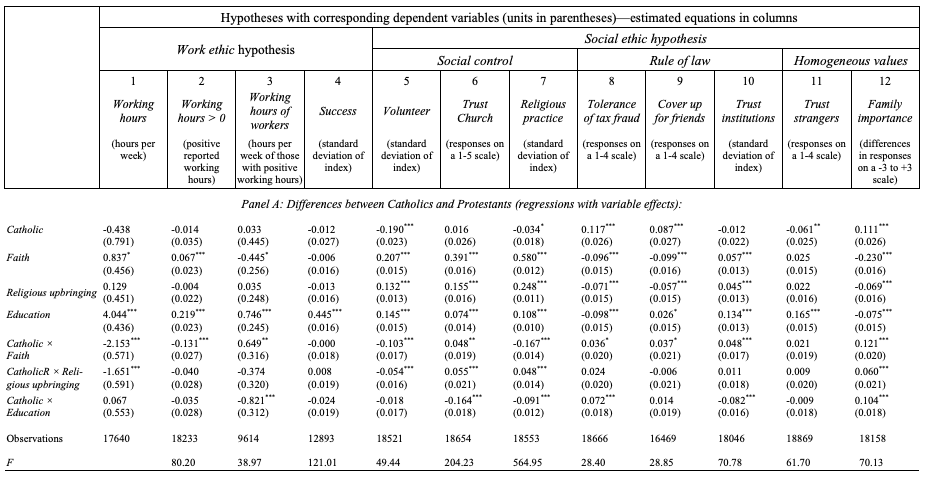
\includegraphics[width=11cm, height=7cm]{hola}
\centering
\end{frame}
%------------------------------------------------
\begin{frame}
\frametitle{Concluding Diferences}
\begin{itemize}
\item The more diverse Catholic moral standards may increase transaction costs in impersonal trading but
also make personal trade easier.
\item Average Catholics trust strangers less.
\item Catholics give more importance than Protestants to family ties.
\end{itemize}
\end{frame}
%------------------------------------------------
\section{Concluding Remarks}
%------------------------------------------------
\begin{frame}
\frametitle{Overall}
\begin{itemize}
\item The consequences for economic growth and the development of Capitalism would be related with:
\end{itemize}
\begin{enumerate}
\item The greater effort that individuals are willing to exert in informal social enforcement.
\item The contribution that having more independent individuals makes to the design and functioning of political and legal
institutions.
\item To the greater homogeneity of values among individuals.
\end{enumerate}
\begin{itemize}
\item These features facilitate legal enforcement and reduce the cost of impersonal exchange. 
\end{itemize}
\end{frame}
%------------------------------------------------
\section{References}
%------------------------------------------------
\begin{frame}
\frametitle{References}
\footnotesize{
\begin{thebibliography}{99} 
\bibitem[Arruñada, 2010]{p1} Benito Arruñada (2010)
\newblock  "Protestants and Catholics: Similar work ethic, different social ethic"
\newblock \emph{The Economic Journal} 120(547), pp.890-918.
\end{thebibliography}
}
\end{frame}
%------------------------------------------------
\begin{frame}
\Huge{\centerline{The End}}
\end{frame}
%------------------------------------------------
\end{document}
